\documentclass[a4paper,10pt]{article}
\setlength{\parindent}{0.5cm}
\setlength{\parskip}{\baselineskip} 

\usepackage{graphicx}
\usepackage[utf8]{inputenc}
\usepackage[spanish]{babel}
\usepackage{color}
\usepackage{placeins}
\usepackage[T1]{fontenc}
\usepackage{listings}

\lstset{ %
language=C++,                % choose the language of the code
basicstyle=\footnotesize,       % the size of the fonts that are used for the code
numbers=left,                   % where to put the line-numbers
numberstyle=\footnotesize,      % the size of the fonts that are used for the line-numbers
stepnumber=1,                   % the step between two line-numbers. If it is 1 each line will be numbered
numbersep=5pt,                  % how far the line-numbers are from the code
backgroundcolor=\color{white},  % choose the background color. You must add \usepackage{color}
showspaces=false,               % show spaces adding particular underscores
showstringspaces=false,         % underline spaces within strings
showtabs=false,                 % show tabs within strings adding particular underscores
frame=single,           % adds a frame around the code
tabsize=2,          % sets default tabsize to 2 spaces
captionpos=b,           % sets the caption-position to bottom
breaklines=true,        % sets automatic line breaking
breakatwhitespace=false,    % sets if automatic breaks should only happen at whitespace
escapeinside={\%*}{*)}          % if you want to add a comment within your code
}

% Creates indexes for Table of Contents, List of Figures, List of Tables and Index
\makeindex


\title{

\includegraphics[width=0.25\textwidth]{content/escudodelauba2uj.jpg}

\includegraphics[width=0.35\textwidth]{content/logofiubabajatm9.jpg}\\[2.5ex] 
\textbf{66:20 Organizaci\'on de Computadoras  
    Trabajo Pr\'actico 1: assembly MIPS
}
}

\author{
	\textbf{Profesor Titular:} \\ 
	Dr. Ing. Jos\'e Luis Hamkalo  \\[2.5ex] 
	\textbf{Docentes:} \\
	Ing. Leandro Santi  \\
	Ing. Hern\'an P\'erez Masci\\
    Ing. Luciano Natale\\[2.5ex]
	\textbf{Alumnos:}								\\ 
    Opromolla, Giovanni \textit{Padr\'on Nro. 87761}				\\
    Tapia, Jimena Soledad \textit{Padr\'on Nro. 88392}				\\[2.5ex]
	\normalsize{2do. Cuatrimestre de 2015}									\\
	\normalsize{66.20 Organizaci\'on de Computadoras  $-$ Pr\'actica Martes}	\\
	\normalsize{Facultad de Ingenier\'ia, Universidad de Buenos Aires}		\\   
}
\date{}

\begin{document}

	\maketitle

\thispagestyle{empty}   % quita el número en la primer página

\begin{abstract}
Con el presente trabajo pr\'actico logramos familiarizarnos con el conjunto de instrucciones MIPS y el concepto de ABI que se utiliza en la c\'atedra.

\end{abstract}

\newpage

%
\renewcommand{\contentsname}{Indice}
\tableofcontents
\addtocontents{toc}{\par\nobreak \mbox{}\hfill{\bf P\'ag.}\par\nobreak}

\newpage

\section{Introducci\'on}
Se va a implementar una funci\'on en MIPS que resuelva la multiplicaci\'on de matrices de n\'umeros en punto flotante de doble precisi\'on. Dicha funci\'on fue previamente desarrollada en lenguaje C como parte en un programa que recibe matrices por entrada est\'andar, las multiplica tomadas de a pares y devuelve el resultado de la multiplicaci\'on por salida est\'andar (stdout).

\subsection{Objetivo}
Transcribir e implementar a lenguaje MIPS una funci\'on multiplicadora de matrices previamente desarrollada en lenguaje C que adem\'as debe resolver la funcionalidad original.

\newpage

\section{An\'alisis del Problema}
Se detalla a continuaci\'on el an\'alisis previo a la resoluci\'on del trabajo pr\'actico, clasificado en temas de inter\'es:

\subsection{Situaci\'on inicial del equipo}
\begin{enumerate}
\item La tecnolog\'ia a utilizar es nueva para los integrantes del equipo.
\item Se requiere la comprensi\'on y manipulaci\'on de la ABI y el conjunto de instrucciones propuesto por la c\'atedra.
\item El lenguaje solicitado para programar la soluci\'on no es de uso diario de los integrantes del equipo.
\end{enumerate}

De este an\'alisis se resolvi\'o inicialmente focalizarse en la comprensi\'on de la ABI y la pr\'actica del lenguaje MIPS.

\subsection{Problem\'atica a Resolver}
Debe mantenerse del desarrollo original aprobado en el trabajo pr\'actico anterior:
\begin{enumerate}
\item Las matrices de entrada pueden estar mal formadas o incompletas, es decir, pueden contener menos cantidad de valores de los esperados por la dimensi\'on definida.
\item La cantidad de matrices de entrada puede no ser par, interrumpiendo el procesamiento normal de datos ya que el mismo pretende ir multiplicando las matrices de a pares.
\item Las dimensiones indicadas pueden tener un formato incorrecto.
\item Las dimensiones de un par de matrices de entrada, o par formado por la matriz resultante del par anterior, pueden ser incompatibles para su multiplicaci\'on.
\end{enumerate}

Se agrega en este trabajo pr\'actico:
\begin{enumerate}
\item El parseo de los archivos de entrada se va a dejar dentro de la implementaci\'on en lenguaje C.
\item El manejo de memoria de las matrices se va a dejar dentro de la implementaci\'on en lenguaje C.
\item El manejo de errores se va a dejar dentro de la implementaci\'on en lenguaje C.
\end{enumerate}

De este an\'alisis se extrajeron nuevas consideraciones para la reutilizaci\'on del desarrollo entregado anteriormente y la implementaci\'on de la funci\'on en MIPS.

\newpage

\section{Diseño e implementaci\'on del programa}


\subsection{Implementaci\'on del programa}

Para construir este trabajo pr\'actico, se mantuvo la separaci\'on de la l\'ogica de parseo de comandos de entrada y la de c\'alculo de multiplicaci\'on de las matrices, propuesta en la soluci\'on de base.\par

Si bien dicha soluci\'on propuesta para el trabajo pr\'actico anterior fue efic\'az y sencilla, se decidi\'o simplificar a\'un m\'as la funci\'on que efect\'ua la multiplicaci\'on para lograr exponer una interf\'az simple entre el m\'odulo desarrollado en C y el m\'odulo desarrollado en MIPS.\par




\subsection{Esquema de diseño}
A continuación se muestra un diagrama simplificado de las relaciones de los header de problema propuesto.

\begin{figure}[htbp]
	    \centering
		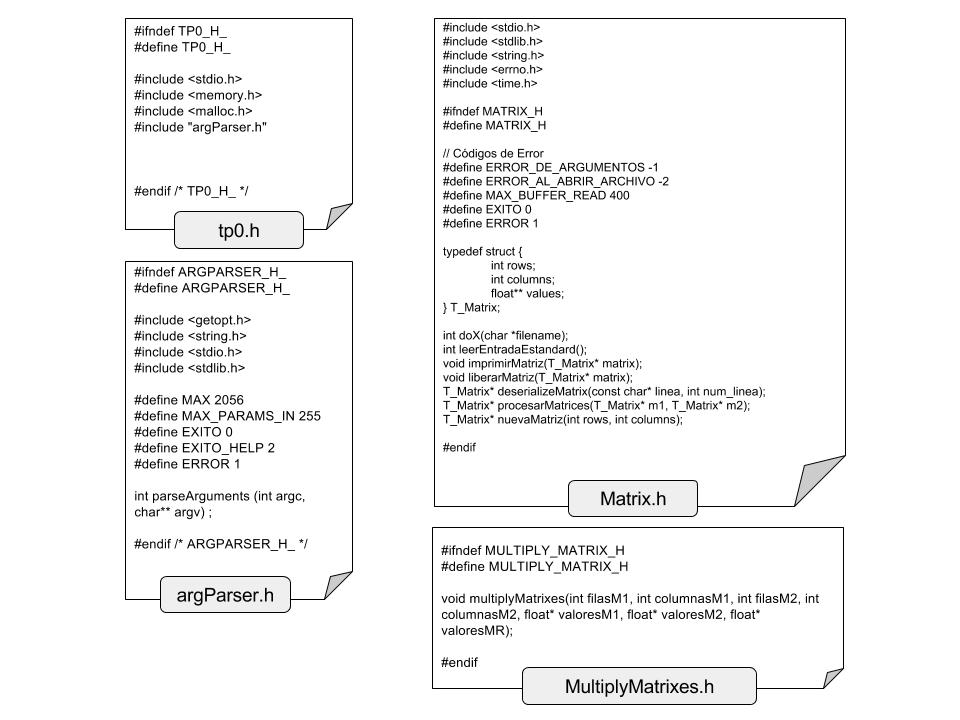
\includegraphics[width=0.90\textwidth]{content/diagrama_h.jpg}
	    \caption{\scriptsize{Diagrama interfaces.}}
	    \label{fig002}
      \end{figure}

\newpage

Y las relaciones de uso entre las mismas.

\begin{figure}[htbp]
	    \centering
		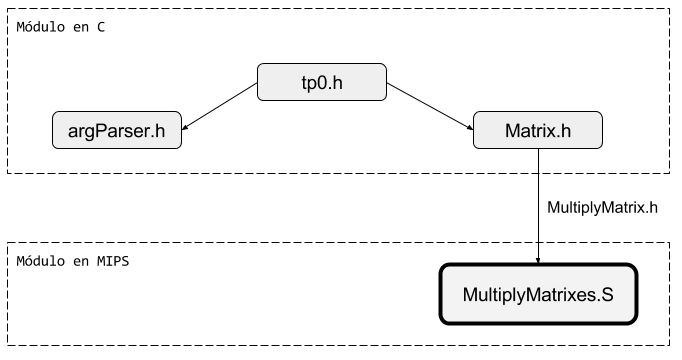
\includegraphics[width=0.90\textwidth]{content/DiagramaRelaciones.png}
	    \caption{\scriptsize{Diagrama Relaciones.}}
	    \label{fig002}
      \end{figure}

\subsection{Funci\'on MIPS}
Para la implementaci\'on del m\'odulo de MIPS se separ\'o primero la l\'ogica relacionada con la multiplicaci\'on de matrices en la funci\'on que se detalla a continuaci\'on, para luego transcribirla a lenguaje MIPS:
\\
\begin{lstlisting}
void multiplyMatrixes(int filasM1, int columnasM1, int filasM2, int columnasM2, float* valoresM1, float* valoresM2, float* valoresMR) {

	int row1, column2,  k;
	float sum;

	for(row1=0; row1<filasM1; ++row1) //filas de la primer matriz
	{
	    for(column2=0; column2<columnasM2; ++column2)  //columnas de la segunda matriz
	    {
	    	sum=0;

	    	for(k=0;k<columnasM1;k++)
	    		sum=sum + valoresM1[(row1*columnasM1) + k] * valoresM2[(k *columnasM2) + column2];

	    	valoresMR[(row1*columnasM2) + column2]=sum;
	    }
	}
}
\end{lstlisting}

El stack para esta funci\'on implementada en MIPS queda como se grafica a continuaci\'on:

\begin{figure}[htbp]
	    \centering
		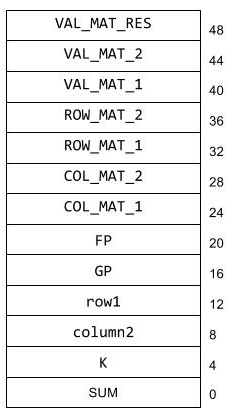
\includegraphics[width=0.50\textwidth]{content/stack_tp1.png}
	    \caption{\scriptsize{Diagrama de stack.}}
	    \label{fig003}
      \end{figure}

\newpage


\section{Compilaci\'on y ejecuci\'on}

Para la compilaci\'on del programa se implement\'o un Makefile como se puede  ver a continuaci\'on:
\\
\begin{lstlisting}[numbers=left,language=bash]
DEPS = \
       src/argParser.h \
       src/MultiplyMatrix.h \
       src/Matrix.h \
       src/tp0.h

OBJ = build/obj/argParser.o \
	  build/obj/MultiplyMatrix.o \
      build/obj/Matrix.o \
      build/obj/tp0.o

VIRTUAL = gxemul-6620-20070927

CC=gcc
CP=cp
CFLAGS=-I./src -Wall $(ACFLAGS)

build: prepare tp0

tp0: $(OBJ)
	gcc -o build/$@ $(OBJ) $(CFLAGS)

build/obj/argParser.o: src/argParser.c $(DEPS)
	$(CC) -c -o $@ src/argParser.c $(CFLAGS)

build/obj/MultiplyMatrix.o: src/MultiplyMatrix.S $(DEPS)
	$(CC) -c -o $@ src/MultiplyMatrix.S $(CFLAGS)

build/obj/Matrix.o: src/Matrix.c $(DEPS)
	$(CC) -c -o $@ src/Matrix.c $(CFLAGS)
	
build/obj/tp0.o: src/tp0.c $(DEPS)
	$(CC) -c -o $@ src/tp0.c $(CFLAGS)

prepare:
	-mkdir -p build
	-mkdir -p build/doc
	-mkdir -p build/obj

clean:
	rm -rf build tags

virtual-start:
	sudo ifconfig lo:0 172.20.0.1
	if [ ! -d ./gxemul/$(VIRTUAL) ]; then bzip2 -dc ./gxemul/$(VIRTUAL).tar.bz2 | cpio --sparse -i -v; mv $(VIRTUAL) ./gxemul/ ; fi
	echo "ssh -f -N -R 2222:127.0.0.1:22 $(USER)@172.20.0.1" | xclip -sel clip
	./gxemul/$(VIRTUAL)/gxemul -e 3max -d ./gxemul/$(VIRTUAL)/netbsd-pmax.img

virtual-reset:
	rm -rf ./gxemul/$(VIRTUAL)

virtual-authkey:
	cat ~/.ssh/id_rsa.pub | ssh -p 2222 root@127.0.0.1 "rm -rf .ssh/authorized_keys; mkdir -p ~/.ssh; cat >> ~/.ssh/authorized_keys"

virtual-deploy:
	ssh -p 2222 root@127.0.0.1 "rm -rf ~/deploy; mkdir -p ~/deploy;"
	scp -P 2222 -r makefile src data root@127.0.0.1:/root/deploy

doc: prepare
	pandoc README.md -o build/doc/README.pdf
	pdflatex --output-directory build/doc docs/informe.tex
	pdflatex --output-directory build/doc docs/informe.tex
	pdflatex --output-directory build/doc docs/informe.tex

doc-preview: doc
	evince build/doc/informe.pdf &

doc-spell:
	aspell -t check docs/informe.tex -d es

export: doc
	tar -czvf build/entrega_tp0.tar.gz makefile src data -C build/doc/ informe.pdf README.pdf

\end{lstlisting}


Para compilar el programa utilizando el Makefile se deben seguir los pasos que se indican en el archivo Readme del proyecto: \\
\begin{lstlisting}[numbers=left,language=bash]
Pasos para correr en la virtual:
$ make virtual-start
login: root
pass: orga6620

Ctrl+Shift+V o copy-paste de la linea "ssh -f -N -R 2222:127.0.0.1:22 giovanni@172.20.0.1"

abrir otra consola y hacer un:
$ make virtual-deploy (despliega los archivos importarntes a la virtual)

ahora volvemos a la consolita anterior y entran en deploy
$ cd deploy/
$ make build
Ahi se les compila todo en MIPS... 

el ejecutable se genera en ~/deploy/build/tp1
los archivos para correr estan bajo la carpeta de data/

Ejemplo de corrida: ~/deploy/$ build/tp1 < data/in1.txt
\end{lstlisting}
\newpage

\section{Pruebas}

Para probar la aplicaci\'on se ejecutaron las pruebas sencillas presentadas a modo de ejemplo en el enunciado del trabajo. \\

\subsection{-h Help}

\begin{lstlisting}[numbers=left,language=bash]
  $ ./build/tp1 -h            
Usage:
  ./tp1 -h
  ./tp1 -V
  ./tp1  < in_file > out_file
Options:
  -V, --version Print version and quit.
  -h, --help    Print this information and quit.
Examples:
  ./tp1 < in.txt > out.txt
  cat in.txt | ./tp1 > out.txt


\end{lstlisting}



\subsection{-V Version}


\begin{lstlisting}[numbers=left,language=bash]
	$ ./build/tp1 -V

        TP1 - assembly MIPS
  (66.20) Organizacion de las Computadoras
------------------------------------------------
        2do Cuatrimestre de 2015
              Version: 1.0

Autores:
         Opromolla, Giovanni - 87761
         Tapia, Jimena Soledad - 88392


\end{lstlisting}


\subsection{build/tp1 < data/in1.txt}
Se realiza una prueba simple, con un archivo que contiene un conjunto de matrices cuyas dimensiones son compatibles para la multiplicaci\'on de a pares. Se muestra el archivo de entrada y el resultado de la ejecuci\'on:

\begin{lstlisting}[numbers=left,language=bash]
2x3 1 2 3 4 5 6.1
3x2 1 0 0 0 0 1
3x3 1 2 3 4 5 6.1 3 2 1
3x1 1 1 0
\end{lstlisting}
\begin{lstlisting}
$ ./build/tp1 < data/in1.txt
2x2 1.000000 3.000000 4.000000 6.100000 
3x1 3.000000 9.000000 5.000000 
\end{lstlisting}

\subsection{build/tp1 < data/in5.txt}
Se realiza una prueba simple, con un archivo que contiene un conjunto de matrices cuyas dimensiones son compatibles para la multiplicaci\'on de a pares. Se muestra el archivo de entrada y el resultado de la ejecuci\'on:

\begin{lstlisting}[numbers=left,language=bash]
4x3 1 2 3 4 5 6 7 8 9 10 11 12
3x1 1 2 3
\end{lstlisting}
\begin{lstlisting}
$ ./build/tp1 < data/in5.txt
4x1 14.000000 32.000000 50.000000 68.000000 
\end{lstlisting}

\subsection{build/tp1 < data/in8.txt}
Se realiza una prueba simple, con un archivo que contiene un conjunto de matrices cuyas dimensiones son compatibles para la multiplicaci\'on de a pares. Se muestra el archivo de entrada y el resultado de la ejecuci\'on:

\begin{lstlisting}[numbers=left,language=bash]
5x5 1 2 3 4 5 6 7 8 9 10 11 12 13 14 15 16 17 18 19 20 21 22 23 24 25
5x5 25 24 23 22 21 20 19 18 17 16 15 14 13 12 11 10 9 8 7 6 5 4 3 2 1.1
\end{lstlisting}
\begin{lstlisting}
./build/tp1 < data/in8.txt
5x5 175.000000 160.000000 145.000000 130.000000 115.499992 550.000000 510.000000 470.000000 430.000000 390.999969 925.000000 860.000000 795.000000 730.000000 666.499939 1300.000000 1210.000000 1120.000000 1030.000000 941.999939 1675.000000 1560.000000 1445.000000 1330.000000 1217.499878
\end{lstlisting}

\subsection{build/tp1 < data/in9.txt}
Se realiza una prueba simple, con un archivo que contiene un varios conjunto de matrices cuyas dimensiones son compatibles para la multiplicaci\'on de a pares. Se muestra el archivo de entrada y el resultado de la ejecuci\'on:

\begin{lstlisting}[numbers=left,language=bash]
5x5 1 2 3 4 5 6 7 8 9 10 11 12 13 14 15 16 17 18 19 20 21 22 23 24 25
5x5 25 24 23 22 21 20 19 18 17 16 15 14 13 12 11 10 9 8 7 6 5 4 3 2 1.1
2x3 1 2 3 4 5 6.1
3x2 1 0 0 0 0 1
5x5 1 2 3 4 5 6 7 8 9 10 11 12 13 14 15 16 17 18 19 20 21 22 23 24 25
5x5 25 24 23 22 21 20 19 18 17 16 15 14 13 12 11 10 9 8 7 6 5 4 3 2 1.1
2x3 1 2 3 4 5 6.1
3x2 1 0 0 0 0 1
5x5 1 2 3 4 5 6 7 8 9 10 11 12 13 14 15 16 17 18 19 20 21 22 23 24 25
5x5 25 24 23 22 21 20 19 18 17 16 15 14 13 12 11 10 9 8 7 6 5 4 3 2 1.1
2x3 1 2 3 4 5 6.1
3x2 1 0 0 0 0 1
5x5 1 2 3 4 5 6 7 8 9 10 11 12 13 14 15 16 17 18 19 20 21 22 23 24 25
5x5 25 24 23 22 21 20 19 18 17 16 15 14 13 12 11 10 9 8 7 6 5 4 3 2 1.1
2x3 1 2 3 4 5 6.1
3x2 1 0 0 0 0 1
5x5 1 2 3 4 5 6 7 8 9 10 11 12 13 14 15 16 17 18 19 20 21 22 23 24 25
5x5 25 24 23 22 21 20 19 18 17 16 15 14 13 12 11 10 9 8 7 6 5 4 3 2 1.1
2x3 1 2 3 4 5 6.1
3x2 1 0 0 0 0 1
5x5 1 2 3 4 5 6 7 8 9 10 11 12 13 14 15 16 17 18 19 20 21 22 23 24 25
5x5 25 24 23 22 21 20 19 18 17 16 15 14 13 12 11 10 9 8 7 6 5 4 3 2 1.1
2x3 1 2 3 4 5 6.1
3x2 1 0 0 0 0 1
5x5 1 2 3 4 5 6 7 8 9 10 11 12 13 14 15 16 17 18 19 20 21 22 23 24 25
5x5 25 24 23 22 21 20 19 18 17 16 15 14 13 12 11 10 9 8 7 6 5 4 3 2 1.1
2x3 1 2 3 4 5 6.1
3x2 1 0 0 0 0 1
5x5 1 2 3 4 5 6 7 8 9 10 11 12 13 14 15 16 17 18 19 20 21 22 23 24 25
5x5 25 24 23 22 21 20 19 18 17 16 15 14 13 12 11 10 9 8 7 6 5 4 3 2 1.1
2x3 1 2 3 4 5 6.1
3x2 1 0 0 0 0 1
5x5 1 2 3 4 5 6 7 8 9 10 11 12 13 14 15 16 17 18 19 20 21 22 23 24 25
5x5 25 24 23 22 21 20 19 18 17 16 15 14 13 12 11 10 9 8 7 6 5 4 3 2 1.1
2x3 1 2 3 4 5 6.1
3x2 1 0 0 0 0 1
5x5 1 2 3 4 5 6 7 8 9 10 11 12 13 14 15 16 17 18 19 20 21 22 23 24 25
5x5 25 24 23 22 21 20 19 18 17 16 15 14 13 12 11 10 9 8 7 6 5 4 3 2 1.1
2x3 1 2 3 4 5 6.1
3x2 1 0 0 0 0 1
5x5 1 2 3 4 5 6 7 8 9 10 11 12 13 14 15 16 17 18 19 20 21 22 23 24 25
5x5 25 24 23 22 21 20 19 18 17 16 15 14 13 12 11 10 9 8 7 6 5 4 3 2 1.1
2x3 1 2 3 4 5 6.1
3x2 1 0 0 0 0 1
5x5 1 2 3 4 5 6 7 8 9 10 11 12 13 14 15 16 17 18 19 20 21 22 23 24 25
5x5 25 24 23 22 21 20 19 18 17 16 15 14 13 12 11 10 9 8 7 6 5 4 3 2 1.1
2x3 1 2 3 4 5 6.1
3x2 1 0 0 0 0 1
5x5 1 2 3 4 5 6 7 8 9 10 11 12 13 14 15 16 17 18 19 20 21 22 23 24 25
5x5 25 24 23 22 21 20 19 18 17 16 15 14 13 12 11 10 9 8 7 6 5 4 3 2 1.1
2x3 1 2 3 4 5 6.1
3x2 1 0 0 0 0 1
5x5 1 2 3 4 5 6 7 8 9 10 11 12 13 14 15 16 17 18 19 20 21 22 23 24 25
5x5 25 24 23 22 21 20 19 18 17 16 15 14 13 12 11 10 9 8 7 6 5 4 3 2 1.1
\end{lstlisting}
\begin{lstlisting}
$ ./build/tp1 < data/in9.txt
5x5 175.000000 160.000000 145.000000 130.000000 115.499992 550.000000 510.000000 470.000000 430.000000 390.999969 925.000000 860.000000 795.000000 730.000000 666.499939 1300.000000 1210.000000 1120.000000 1030.000000 941.999939 1675.000000 1560.000000 1445.000000 1330.000000 1217.499878 
2x2 1.000000 3.000000 4.000000 6.100000 
5x5 175.000000 160.000000 145.000000 130.000000 115.499992 550.000000 510.000000 470.000000 430.000000 390.999969 925.000000 860.000000 795.000000 730.000000 666.499939 1300.000000 1210.000000 1120.000000 1030.000000 941.999939 1675.000000 1560.000000 1445.000000 1330.000000 1217.499878 
2x2 1.000000 3.000000 4.000000 6.100000 
5x5 175.000000 160.000000 145.000000 130.000000 115.499992 550.000000 510.000000 470.000000 430.000000 390.999969 925.000000 860.000000 795.000000 730.000000 666.499939 1300.000000 1210.000000 1120.000000 1030.000000 941.999939 1675.000000 1560.000000 1445.000000 1330.000000 1217.499878 
2x2 1.000000 3.000000 4.000000 6.100000 
5x5 175.000000 160.000000 145.000000 130.000000 115.499992 550.000000 510.000000 470.000000 430.000000 390.999969 925.000000 860.000000 795.000000 730.000000 666.499939 1300.000000 1210.000000 1120.000000 1030.000000 941.999939 1675.000000 1560.000000 1445.000000 1330.000000 1217.499878 
2x2 1.000000 3.000000 4.000000 6.100000 
5x5 175.000000 160.000000 145.000000 130.000000 115.499992 550.000000 510.000000 470.000000 430.000000 390.999969 925.000000 860.000000 795.000000 730.000000 666.499939 1300.000000 1210.000000 1120.000000 1030.000000 941.999939 1675.000000 1560.000000 1445.000000 1330.000000 1217.499878 
2x2 1.000000 3.000000 4.000000 6.100000 
5x5 175.000000 160.000000 145.000000 130.000000 115.499992 550.000000 510.000000 470.000000 430.000000 390.999969 925.000000 860.000000 795.000000 730.000000 666.499939 1300.000000 1210.000000 1120.000000 1030.000000 941.999939 1675.000000 1560.000000 1445.000000 1330.000000 1217.499878 
2x2 1.000000 3.000000 4.000000 6.100000 
5x5 175.000000 160.000000 145.000000 130.000000 115.499992 550.000000 510.000000 470.000000 430.000000 390.999969 925.000000 860.000000 795.000000 730.000000 666.499939 1300.000000 1210.000000 1120.000000 1030.000000 941.999939 1675.000000 1560.000000 1445.000000 1330.000000 1217.499878 
2x2 1.000000 3.000000 4.000000 6.100000 
5x5 175.000000 160.000000 145.000000 130.000000 115.499992 550.000000 510.000000 470.000000 430.000000 390.999969 925.000000 860.000000 795.000000 730.000000 666.499939 1300.000000 1210.000000 1120.000000 1030.000000 941.999939 1675.000000 1560.000000 1445.000000 1330.000000 1217.499878 
2x2 1.000000 3.000000 4.000000 6.100000 
5x5 175.000000 160.000000 145.000000 130.000000 115.499992 550.000000 510.000000 470.000000 430.000000 390.999969 925.000000 860.000000 795.000000 730.000000 666.499939 1300.000000 1210.000000 1120.000000 1030.000000 941.999939 1675.000000 1560.000000 1445.000000 1330.000000 1217.499878 
2x2 1.000000 3.000000 4.000000 6.100000 
5x5 175.000000 160.000000 145.000000 130.000000 115.499992 550.000000 510.000000 470.000000 430.000000 390.999969 925.000000 860.000000 795.000000 730.000000 666.499939 1300.000000 1210.000000 1120.000000 1030.000000 941.999939 1675.000000 1560.000000 1445.000000 1330.000000 1217.499878 
2x2 1.000000 3.000000 4.000000 6.100000 
5x5 175.000000 160.000000 145.000000 130.000000 115.499992 550.000000 510.000000 470.000000 430.000000 390.999969 925.000000 860.000000 795.000000 730.000000 666.499939 1300.000000 1210.000000 1120.000000 1030.000000 941.999939 1675.000000 1560.000000 1445.000000 1330.000000 1217.499878 
2x2 1.000000 3.000000 4.000000 6.100000 
5x5 175.000000 160.000000 145.000000 130.000000 115.499992 550.000000 510.000000 470.000000 430.000000 390.999969 925.000000 860.000000 795.000000 730.000000 666.499939 1300.000000 1210.000000 1120.000000 1030.000000 941.999939 1675.000000 1560.000000 1445.000000 1330.000000 1217.499878 
2x2 1.000000 3.000000 4.000000 6.100000 
5x5 175.000000 160.000000 145.000000 130.000000 115.499992 550.000000 510.000000 470.000000 430.000000 390.999969 925.000000 860.000000 795.000000 730.000000 666.499939 1300.000000 1210.000000 1120.000000 1030.000000 941.999939 1675.000000 1560.000000 1445.000000 1330.000000 1217.499878 
2x2 1.000000 3.000000 4.000000 6.100000 
5x5 175.000000 160.000000 145.000000 130.000000 115.499992 550.000000 510.000000 470.000000 430.000000 390.999969 925.000000 860.000000 795.000000 730.000000 666.499939 1300.000000 1210.000000 1120.000000 1030.000000 941.999939 1675.000000 1560.000000 1445.000000 1330.000000 1217.499878 
\end{lstlisting}

\subsection{build/tp1 < data/in2.txt}
Se realiza una prueba con un archivo que contiene un conjunto de matrices cuyas dimensiones no son compatibles para la multiplicaci\'on de a pares. Se muestra el archivo de entrada y el resultado de la ejecuci\'on:

\begin{lstlisting}[numbers=left,language=bash]
2x2 1 3 4 6.1
3x1 3 9 5
\end{lstlisting}
\begin{lstlisting}
$ build/tp1 < data/in2.txt
Las propiedades de multiplicacion de matrices no estan satisfechas.
\end{lstlisting}

\subsection{build/tp1 < data/in3.txt}
Se realiza una prueba con un archivo que contiene datos con formato incorrecto. No se respeta el formato de entrada acordado "NxM a1,1 a1,2 ... a1,M a2,1 a2,2 ... a2,M ... aN,1 aN,2 ... aN,M". Se muestra el archivo de entrada y el resultado de la ejecuci\'on:

\begin{lstlisting}[numbers=left,language=bash]
12xx 12351
\end{lstlisting}
\begin{lstlisting}
$ build/tp1 < data/in3.txt
Error al leer los valores de NxM en la linea 0.
\end{lstlisting}

\subsection{build/tp1 < data/in4.txt}
Se realiza una prueba con un archivo que contiene matrices incompletas, es decir, que las dimensiones indicadas no se corresponden con los valores aX,Y listados. Se muestra el archivo de entrada y el resultado de la ejecuci\'on:

\begin{lstlisting}[numbers=left,language=bash]
2x2 1.1 2.2 3.3
\end{lstlisting}
\begin{lstlisting}
$ build/tp1 < data/in4.txt
Faltan valores en la matriz de 2x2 de la linea 0.
\end{lstlisting}

\subsection{build/tp1 < data/in7.txt}
Se realiza una prueba con un archivo que contiene matrices con letras en vez de n\'umeros, es decir, el formato de dato no es el esperado. Se muestra el archivo de entrada y el resultado de la ejecuci\'on:

\begin{lstlisting}[numbers=left,language=bash]
2x2 1 2 3 4
2x2 1 d 3 4
\end{lstlisting}
\begin{lstlisting}
./build/tp1 < data/in7.txt
Valores invalidos en la matriz de 2x2 de la linea 1.
\end{lstlisting}

\newpage

\section{Manejo de errores}
Para manejar errores y advertirle al usuario de los mismos se utilizaron mensajes por linea de comando:\\

\subsection{Comando inexistente}
En este caso se eligió mostrar el menú de opciones para que el usuario pueda seleccionar un comando correcto, dentro de los entendidos por el programa.

\begin{lstlisting}[language=bash]
$ build/tp0 -u

build/tp1: invalid option -- 'u'
Usage:
  ./tp1 -h
  ./tp1 -V
  ./tp1  < in_file > out_file
Options:
  -V, --version	Print version and quit.
  -h, --help	Print this information and quit.
Examples:
  ./tp1 < in.txt > out.txt
  cat in.txt | ./tp0 > out.txt
  
\end{lstlisting}
\newpage


\section{Conclusiones}
Con el desarrollo del presente trabajo pr\'actico pusimos en pr\'actica la codificaci\'on en assembly MIPS y la comprensi\'on de la conformaci\'on del stack para la funci\'on implementada. Lo que nos result\'o de mayor complejidad fue el manejo de datos de tipo float. Nos encontramos tambi\'en con problemas para el acceso y modificaci\'on de las matrices, pero logramos corregirlos ya que se deb\'ieron a un error en la instrucci\'on utilizada para manejo de array.\\


\newpage

\section{C\'odigo}


\subsection{C\'odigo C}
\title{argParser.h}
\begin{lstlisting}[language=C]

#ifndef ARGPARSER_H_
#define ARGPARSER_H_

#include <getopt.h>
#include <string.h>
#include <stdio.h>
#include <stdlib.h>

#define MAX 2056
#define MAX_PARAMS_IN 255
#define EXITO 0
#define EXITO_HELP 2
#define ERROR 1

int parseArguments (int argc, char** argv) ;

#endif /* ARGPARSER_H_ */

\end{lstlisting}

\title{argParser.c}
\begin{lstlisting}[language=C]
#include "argParser.h"

int showMenuHelp()
{
    printf("Usage:\n");
    printf("  ./tp1 -h\n");
    printf("  ./tp1 -V\n");
    printf("  ./tp1  < in_file > out_file\n");
    printf("Options:\n");
    printf("  -V, --version\tPrint version and quit.\n");
    printf("  -h, --help\tPrint this information and quit.\n");
    printf("Examples:\n");
    printf("  ./tp1 < in.txt > out.txt\n");
    printf("  cat in.txt | ./tp1 > out.txt\n");
    return EXITO;
}

int showMenuVersion()
{
	printf("\n\tTP1 - assembly MIPS\n");
	printf("  (66.20) Organizacion de las Computadoras\n");
 	printf("------------------------------------------------\n");
	printf("\t2do Cuatrimestre de 2015\n");
	printf("\t      Version: 1.0\n");
	printf("\nAutores:\n");
	printf("         Opromolla, Giovanni - 87761\n");
	printf("         Tapia, Jimena Soledad - 88392\n\n");
	return EXITO;

}


int readOptions (int argc, char** argv, const char* op_cortas, const struct option op_largas[]) {

	int siguiente_opcion = 0;
	int result = ERROR;

	siguiente_opcion = getopt_long(argc, argv, op_cortas, op_largas, NULL);

	switch (siguiente_opcion) {
		case 'h' : /* -h o --help */
			showMenuHelp();
			result = EXITO_HELP;
			break;
		case 'V' : /* -V o --version */
			showMenuVersion();
			result = EXITO_HELP;
			break;
		case '?' : /* opcion no valida */
			showMenuHelp();
			result = EXITO_HELP;
			break;
		default : /* Algo mas? No esperado. Abortamos */
			result = EXITO;
	}

	return result;
}



int parseArguments (int argc, char** argv) {
  
	int result = ERROR;
		
	/* Una cadena que lista las opciones cortas validas */
	const char* op_cortas = "hV" ;

	/* Una estructura de varios arrays describiendo los valores largos */
	const struct option op_largas[] = {
		{ "help",         0,  NULL,   'h'},
		{ "version",      0,  NULL,   'V'},
		{ NULL,           0,  NULL,   0  }
	};

	result = readOptions(argc, argv, op_cortas, op_largas);
	
	if(result == ERROR){
	    showMenuHelp();
	}
	
	return result;
}

\end{lstlisting}

\title{Matrix.h}
\begin{lstlisting}[language=C]
#include <stdio.h>
#include <stdlib.h>
#include <string.h>
#include <errno.h>
#include <time.h>
#include <ctype.h>

#ifndef MATRIX_H
#define MATRIX_H

// Codigos de Error
#define ERROR_DE_ARGUMENTOS -1
#define ERROR_AL_ABRIR_ARCHIVO -2
#define MAX_BUFFER_READ 400
#define EXITO 0
#define ERROR 1

typedef struct {
	int rows;
	int columns;
	float* values;
} T_Matrix;

int doX(char *filename);
int leerEntradaEstandard();
int isDigit(char* str);
void imprimirMatriz(T_Matrix* matrix);
void liberarMatriz(T_Matrix* matrix);

T_Matrix* deserializeMatrix(const char* linea, int num_linea);
T_Matrix* procesarMatrices(T_Matrix* m1, T_Matrix* m2);
T_Matrix* nuevaMatriz(int rows, int columns);

#endif

\end{lstlisting}
\title{Matrix.c
\begin{lstlisting}[language=C]
#include "Matrix.h"
#include "MultiplyMatrix.h"
#define BUF_SIZE 255

int leerEntradaEstandard()
{

    char line[BUF_SIZE];
    int num_linea = 0;

    T_Matrix* m1 = NULL;
    T_Matrix* m2 = NULL;
    T_Matrix* m_resultado = NULL;
    /** Lectura de stdin para obtener las matrices linea por linea **/

    while((fgets(line,BUF_SIZE,stdin)) != NULL){

    	if(strlen(line) > 2){
			if (num_linea%2 == 0)		/** Pares **/
			{
				m1 = deserializeMatrix(line, num_linea);
				if (m1 == NULL) {
          /** Algun problema surgio al deserealizar la matriz **/
          fprintf(stderr, "Ocurrio un error al procesar una las lineas. Verique el formato y la cantidad de matrices en el archivo.\n");
  				break;
        }
			}
			else						/** Impares **/
			{
				m2 = deserializeMatrix(line, num_linea);
				if (m2 == NULL){
				  liberarMatriz(m1);
          fprintf(stderr, "Ocurrio un error al procesar una las lineas. Verique el formato y la cantidad de matrices en el archivo.\n");
          break;
        } 	/** Algun problema surgio al deserealizar la matriz **/
				else{
					m_resultado = procesarMatrices(m1, m2);

					if(m_resultado != NULL)
						imprimirMatriz(m_resultado);

					liberarMatriz(m1);
					liberarMatriz(m2);
					liberarMatriz(m_resultado);
				}
			}
			++num_linea;
    	}
	}

    return EXITO;
}

void imprimirMatriz(T_Matrix* matrix){
	int pos;
  printf("%dx%d ", matrix->rows, matrix->columns);
	for (pos=0; pos < (matrix->rows*matrix->columns); pos++)
	{
	    printf("%f ", matrix->values[pos]);
	}
  printf("\n");
}

void liberarMatriz(T_Matrix* matrix){

	free( matrix->values );
	free(matrix);
	matrix = NULL;
}


char* serializeMatrix(T_Matrix* m ){
    char* matrix_str = NULL;

    return matrix_str;
}

int isDigit(char* str){
	int i,res = EXITO, len = strlen(str);

	for(i=0; i < len; ++i)
	{
		if(isalpha(str[i]))
		{
			res = ERROR;
			break;
		}
	}

	return res;
}

T_Matrix* deserializeMatrix(const char* linea, int num_linea){

	int rows = -1;
	int columns = -1;
	int val = sscanf(linea, "%dx%d", &rows, &columns);

	/** Verificar que se hayan podido leer ambos valores **/
	if (val != 2)
	{
		fprintf(stderr, "Error al leer los valores de NxM en la linea %d.\n", num_linea);
		exit(1);
	}
	/** Verificar que ambos valores sean mayores a cero **/
	if((rows < 0) || (columns < 0)){
		fprintf(stderr, "Los valres de NxM deben ser valores positivos. Linea conflictiva: %d.\n", num_linea);
		exit(1);
	}

	/** Creo matriz y aloco su memoria **/
	T_Matrix* matrix = nuevaMatriz(rows, columns);

	/** Obtengo los valores de la matriz **/
    char* valores = strstr (linea," ");;
    char *token;
    token = strtok(valores, " ");

    
    int f=0, c=0;
    while( (token != NULL) && (f < rows ) )
    {
    	if( isDigit(token) == EXITO){
    		matrix->values[(f*columns)+c] = atof(token);
    		token = strtok(NULL, " ");
    		if(f < rows){
    			c++;
    			if(c == columns){
    				f++;
    				c = 0;
    			}
    		}
    	}
    	else{
        	fprintf(stderr, "Valores invalidos en la matriz de %dx%d de la linea %d.\n", matrix->rows, matrix->columns, num_linea );
        	liberarMatriz(matrix);
        	exit(1);
    	}
    }
    
    /** Matriz incompleta **/
    if(f != rows){
    	fprintf(stderr, "Faltan valores en la matriz de %dx%d de la linea %d.\n", matrix->rows, matrix->columns, num_linea );
    	liberarMatriz(matrix);
    	exit(1);
    }

    /** Imprimo la matriz **/
    //imprimirMatriz(matrix);

	return matrix;
}

T_Matrix* nuevaMatriz(int rows, int columns){

	T_Matrix* matrix = (T_Matrix*) malloc(sizeof (T_Matrix) );

	matrix->rows = rows;
	matrix->columns = columns;

	/** Aloco espacio para la matriz **/
	matrix->values = (float*) malloc (sizeof(float)*matrix->rows*matrix->columns);

	return matrix;
}

T_Matrix* procesarMatrices(T_Matrix* m1, T_Matrix* m2){

	T_Matrix* matrix = NULL;

	if(m1->columns == m2->rows) {
		/** Creo matriz y aloco su memoria **/
		matrix = nuevaMatriz(m1->rows, m2->columns);

		multiplyMatrixes(m1->rows, m1->columns, m2->rows, m2->columns, m1->values, m2->values, matrix->values);

	}else{
    	fprintf(stderr, "Las propiedades de multiplicacion de matrices no estan satisfechas.\n");
    	exit(1);
	}

	return matrix;

}



\end{lstlisting}


\title{tp0.h}
\begin{lstlisting}[language=C]
/*
 * tp0.h
 *
 *  Created on: Sep 9, 2015
 *      Author: giovanni
 */

#ifndef TP0_H_
#define TP0_H_

#include <stdio.h>
#include <memory.h>
#include <malloc.h>
#include "argParser.h"



#endif /* TP0_H_ */

\end{lstlisting}

\title{tp0.c}
\begin{lstlisting}[language=C]
#include "tp0.h"
#include "Matrix.h"

int main(int argc, char** argv){
	
      int result = parseArguments(argc, argv);
            
      if(result == 0)
	  result = leerEntradaEstandard();
      else if (result == 1)
	  perror("Error al obtener los argumentos.");
            
      return 0;
}
\end{lstlisting}

\title{MultiplyMatrixes.h}
\begin{lstlisting}[language=C]
#include <stdio.h>
#include <stdlib.h>
#include <string.h>
#include <errno.h>
#include <time.h>

#ifndef MULTIPLY_MATRIX_H
#define MULTIPLY_MATRIX_H

void multiplyMatrixes(int filasM1, int columnasM1, int filasM2, int columnasM2, float* valoresM1, float* valoresM2, float* valoresMR);

#endif

\end{lstlisting}


\subsection{C\'odigo MIPS}

\title{MultiplyMatrixes.S}
\begin{lstlisting}[language=C]
#include <mips/regdef.h>
#include <sys/syscall.h>

#define SF 24
#define FP 20
#define GP 16
#define fp $30

#define COL_MAT_1 24
#define COL_MAT_2 28
#define ROW_MAT_1 32
#define ROW_MAT_2 36
#define VAL_MAT_1 40
#define VAL_MAT_2 44
#define VAL_MAT_RES 48   
#define ROW1 12
#define COL2 8
#define K 4
#define SUM 0 

.text
.align 2


.globl  multiplyMatrixes
.ent    multiplyMatrixes

multiplyMatrixes:
        .frame  fp,SF,ra
        .set    noreorder
        .cpload t9
        .set    reorder

        #stack frame creation
        subu    sp,sp,SF

        .cprestore GP
        sw fp, FP(sp)
        move fp, sp
        
        #Guardo los argumentos
        sw a0, ROW_MAT_1(fp)       # FilasM1
        sw a1, COL_MAT_1(fp)       # ColumnasM1
        sw a2, ROW_MAT_2(fp)       # FilasM2
        sw a3, COL_MAT_2(fp)       # ColumnasM2
    	#    sw t7, VAL_MAT_1(fp)       # ValuesM1
   	#    sw t8, VAL_MAT_2(fp)       # ValuesM2
  	#    sw t9, VAL_MAT_RES(fp)     # ValuesMR

		sw zero, ROW1(fp)			# row1 = 0
		lw t0, ROW_MAT_1(fp)		# t0 = filasM1
		lw t1, ROW1(fp)			# t1 = row1
		
FOR_ROWS:								# for(row1=0# row1<filasM1# ++row1)
		beq 	t1, t0, EXIT_FOR_ROWS 	# if row1 == filas1 we are done
		sw		zero, COL2(fp)			# col2 = 0
		lw		t2, COL_MAT_2(fp)		# t2 = ColumnasM2
		lw		t3, COL2(fp)			# t3 = column2

FOR_COLS:
		beq		t3, t2, EXIT_FOR_COLS	# for(column2=0# column2<columnasM2# ++column2)
		sw		zero, SUM(fp)			# sum = 0
		l.s		$f4, SUM(fp)
		sw		zero, K(fp) 			# k=0
		lw		t4, COL_MAT_1(fp)		# t4 = ColumnasM1
		lw		t5, K(fp)				# t5 = k
		#j EXIT_FOR_SUM
FOR_SUM:
		beq		t5, t4, EXIT_FOR_SUM	# for(k=0# k<columnasM1# k++)
		#valoresM1[(row1*columnasM1) + k]
		lw	t6, VAL_MAT_1(fp )		# valoresM1
		mul		t7, t1, t4				# t7 = row1*columnasM1
		addu	t7, t7, t5				# t7 = (row1*columnasM1) + k
		sll		t7, t7, 2				# Aligned t7 * 4
		addu	t6, t6, t7				# valoresM1[(row1*columnasM1) + k]
		l.s   	$f0, 0(t6)				# f0 = valoresM1[(row1*columnasM1) + k]
		#valoresM2[(k *columnasM2) + column2]
		lw	t6, VAL_MAT_2(fp)			# valoresM2
		mul		t7, t5, t2				# t7 = k *columnasM2
		addu	t7, t7, t3				# (k *columnasM2) + column2
		sll		t7, t7, 2				# Aligned t7 * 4
		addu	t6, t6, t7				# valoresM2[(k *columnasM2) + column2]
		l.s   	$f2, 0(t6)					# f1 = valoresM2[(k *columnasM2) + column2]
		#sum=sum + valoresM1[(row1*columnasM1) + k] * valoresM2[(k *columnasM2) + column2]#
		mul.s	$f6, $f0, $f2				# valoresM1[(row1*columnasM1) + k] * valoresM2[(k *columnasM2) + column2]
		add.s	$f4, $f4, $f6				# sum=sum + valoresM1[(row1*columnasM1) + k] * valoresM2[(k *columnasM2) + column2]#
		s.s		$f4, SUM(fp)				#
		addi 	t5, t5, 1 				# add 1 to t5 (k)
		j FOR_SUM						# jump back to the top

EXIT_FOR_SUM:
		#valoresMR[(row1*columnasM2) + column2]=sum#
		lw    t6, VAL_MAT_RES(fp)
		#addu	t6, fp, VAL_MAT_RES		# valoresMR
		mul		t7, t1, t2				# t7 = row1*columnasM2
		addu	t7, t7, t3				# t7 = (row1*columnasM2) + column2
		sll		t7, t7, 2				# Aligned t7 * 4
		addu	t6, t6, t7				# t6 = valoresMR[(row1*columnasM2) + column2]
		l.s		$f4, SUM(fp)				# f4 = sum
		s.s		$f4, 0(t6)					# valoresMR[(row1*columnasM2) + column2] = sum
		addi 	t3, t3, 1 				# add 1 to t3 (column2)
		j FOR_COLS						# jump back to the top

EXIT_FOR_COLS:
		addi 	t1, t1, 1 				# add 1 to t1 (row1)
		j FOR_ROWS						# jump back to the top

EXIT_FOR_ROWS:
		move	sp, fp
		lw	fp, FP(sp)
		lw	gp, GP(sp)

		addu	sp, sp, SF
		j	ra

.end multiplyMatrixes



\end{lstlisting}

\newpage
\begin{thebibliography}{99}
\bibitem {gxemul} GXemul,http://gavare.se/gxemul/.
\bibitem {The NetBSD project} The NetBSD project, http://www.netbsd.org/.
\end{thebibliography}
\end{document}

